\documentclass[11pt]{article}

\usepackage[utf8]{inputenc}
\usepackage[T1]{fontenc}
\usepackage[a4paper,margin=2.6cm]{geometry}
\usepackage{amsmath,amssymb,amsthm}
\usepackage{graphicx}
\usepackage{booktabs}
\usepackage{xcolor}
\usepackage{caption}
\usepackage{subcaption}
\usepackage[expansion=false]{microtype}
\usepackage[colorlinks=true,linkcolor=black,citecolor=black,urlcolor=blue]{hyperref}
\usepackage{authblk}
\usepackage{titlesec}

% -- Noms francais (babel-french indisponible sur certaines installations TeX).
%    Si babel-french EST disponible chez toi, tu peux remplacer ce bloc par
%    \usepackage[french]{babel} et supprimer les \renewcommand ci-dessous.
\renewcommand{\abstractname}{R\'esum\'e}
\renewcommand{\refname}{R\'ef\'erences}
\renewcommand{\figurename}{Figure}
\renewcommand{\tablename}{Tableau}
% -- tolerance de justification (pas de motifs de cesure francais)
\tolerance=1200
\emergencystretch=2em
\hyphenation{ar-chi-tec-ture ar-chi-tec-tures com-por-te-ment com-por-te-men-tale
  com-por-te-men-tales m\'e-moire r\'e-cu-p\'e-ra-tion in-ter-ac-tion in-ter-ac-tions
  pr\'e-en-re-gis-tr\'e ex-p\'e-rience ex-p\'e-riences at-trac-teurs
  d\'e-pen-dance trans-mis-sion per-cep-tion cou-pla-ge ex-pli-cite
  in-ter-pr\'e-ta-tion con-fi-gu-ra-tion d\'e-ploie-ment}

\titleformat{\section}{\normalfont\large\bfseries}{\thesection}{0.7em}{}
\titleformat{\subsection}{\normalfont\normalsize\bfseries}{\thesubsection}{0.7em}{}
\captionsetup{font=small,labelfont=bf}

\newcommand{\xa}{x_{A}}
\newcommand{\clip}{\operatorname{clip}}

\title{\bfseries Des effets d'ordre sans attracteurs :\\[0.25em]
\large une échelle d'architectures mémoire pré-enregistrée
pour les agents LLM}

\author[ ]{Adrien Morelle}
\affil[ ]{\small Chercheur indépendant \\ \texttt{https://github.com/Dr1mS/Prototypos}}
\date{\small 23 juillet 2026}

\begin{document}
\maketitle

\begin{abstract}
\noindent
Les agents fondés sur des modèles de langage sont de plus en plus souvent dotés d'une
mémoire persistante, et une littérature grandissante documente leur \emph{dérive}
comportementale au fil d'interactions longues. Nous cherchons à savoir ce qui la
\emph{gouverne}. Sous un protocole pré-enregistré, dont les règles de décision ont été
gelées avant toute collecte de données, nous comparons une échelle d'architectures
mémoire --- sans mémoire, journal brut en ajout seul, mémoire récurrente
auto-résumée, mémoire vectorielle sémantique --- à un agent doté d'un état explicite
de faible dimension couplé à la \emph{perception}. Deux propriétés habituellement
confondues sous le terme de « dérive » se séparent nettement. La
\textbf{dépendance à l'ordre} est gouvernée par l'adressage de la récupération : une
mémoire adressée par contenu transmet l'histoire précoce jusqu'au comportement final
($|r| = 0{,}75$, $99{,}5^\text{e}$ percentile d'un modèle nul de marche aléatoire
apparié), là où les mémoires à fenêtre de récence et à réécriture l'effacent
($3{,}7^\text{e}$ et $78{,}2^\text{e}$). La journalisation des récupérations expose le
mécanisme directement : les exemplaires précoces occupent encore $58\,\%$ des slots
récupérés après une salve corrective complète, soit $1{,}36$ fois leur taux de base
positionnel. La \textbf{structure d'attracteurs}, elle, ne suit pas : toute
architecture naturelle testée est monostable et corrigible --- sur trois modèles dont
un dépourvu de sa direction de refus --- et la correction comportementale
\emph{devance} la composition de la mémoire ; seul l'état explicite couplé à la
perception produit des bassins larges, bimodaux et hystérétiques. Enfin, une
observation non prédite et directement pertinente pour le déploiement : l'agent le
moins prudent est celui qui n'a rien vécu du tout --- après trente-cinq tours coopératifs
ordinaires, les agents obtempèrent sur la moitié d'une batterie de garde-fous, tandis
qu'une mémoire de pression sociale, \emph{quelle qu'en soit la direction}, élève leur
niveau de vigilance. Nous concluons que la dérive comportementale structurée est une
propriété architecturale, et non une conséquence émergente de la persistance mémoire.
\end{abstract}

\vspace{0.5em}

\section{Introduction}

Un agent fondé sur un modèle de langage et doté d'une mémoire persistante conditionne
chacune de ses réponses à une trace de ce qui a précédé. L'attente naturelle est que
cela rende son comportement \emph{dépendant du chemin} : les interactions précoces
devraient façonner de manière disproportionnée la conduite ultérieure, et l'agent
devrait pouvoir s'installer dans des modes comportementaux stables qui résistent à la
correction. Cette attente sous-tend une grande part des préoccupations relatives au
déploiement d'agents sur horizon long, où un assistant peut accumuler des centaines de
tours d'historique avant d'entreprendre une action conséquente.

Nous mettons cette attente à l'épreuve et l'infirmons en grande partie. Notre
observation centrale est que deux phénomènes couramment réunis sous le mot « dérive »
sont en réalité séparables et relèvent de causes architecturales distinctes :

\begin{enumerate}\itemsep0.15em
\item La \textbf{transmission de l'ordre} --- le fait que le \emph{moment} où quelque
chose s'est produit laisse une trace dans le comportement final --- est gouvernée par
la manière dont la mémoire est \emph{adressée}.
\item La \textbf{formation d'attracteurs} --- le fait que le comportement se fixe dans
des bassins larges, stables et résistants à la correction --- n'apparaît dans aucune
architecture mémoire naturelle que nous ayons testée, et requiert un état explicite de
faible dimension couplé à la perception.
\end{enumerate}

\paragraph{Contributions.}
(i) Une échelle d'architectures pré-enregistrée isolant l'adressage de la récupération
comme dimension opérante des effets d'ordre (\S\ref{sec:ladder}).
(ii) La mesure directe, au niveau du récupérateur, du mécanisme qui transmet
l'histoire précoce --- et la démonstration que transmission n'implique pas
verrouillage (\S\ref{sec:transmission}).
(iii) Une observation non prédite, pertinente pour le déploiement : une mémoire
coopérative sans pression constitue l'état le \emph{moins} prudent
(\S\ref{sec:mundane}).
(iv) Une méthode de « champ d'appréciation » peu coûteuse, et la valeur diagnostique
de son échec sur les agents naturels (\S\ref{sec:methods}).

\section{Travaux liés}

\paragraph{Dérive de persona et d'identité.}
Li et al.~\cite{li2024persona} ont introduit un test quantitatif de stabilité de
persona reposant sur des auto-conversations entre agents personnalisés, et rapportent
une dérive significative en moins de huit tours sur LLaMA2-chat-70B, qu'ils attribuent
en partie à la décroissance de l'attention au fil des échanges longs. Choi
et al.~\cite{choi2024identity} ont examiné la cohérence identitaire sur neuf modèles
et constatent que les modèles les plus grands dérivent davantage, et qu'assigner une
persona ne suffit pas à l'empêcher. Le plus proche de notre cadre,
ContextEcho~\cite{contextecho2026} mesure la dérive de persona à l'échelle du
déploiement, sur de longues sessions de codage agentique, au moyen d'un protocole de
capture-puis-sondage qui bifurque l'état conversationnel sans perturber la session
principale --- la discipline de mesure que nous adoptons également
(\S\ref{sec:ladder}).

\paragraph{La mémoire comme source de changement comportemental.}
Dabas et al.~\cite{dabas2026tooldrift} étudient la \emph{dérive d'outillage induite
par la mémoire} : des biais stockés en mémoire affectent silencieusement les appels
d'outils dans des contextes où ils ne s'appliquent pas. Ils rapportent que les
mémoires biaisées agissent comme des vecteurs de pilotage implicites, et que les
défenses standard réduisent l'effet sans l'éliminer. Wei
et al.~\cite{wei2025amemguard} décrivent un cycle d'erreur auto-renforçant dans lequel
un résultat corrompu est stocké comme précédent, amplifiant l'erreur initiale et
abaissant progressivement le seuil de défaillances similaires. Lin
et al.~\cite{lin2026survey} passent en revue la sécurité de la mémoire à long terme et
reformulent la question directrice : non plus « l'entrée actuelle est-elle nuisible ? »
mais « dans quel \emph{état} mémoriel le système se trouve-t-il ? ».

\paragraph{Positionnement de ce travail.}
Cette littérature est majoritairement adversariale ou orientée mesure : elle étudie
des mémoires injectées ou empoisonnées, et mesure la dérive dans des systèmes en boîte
noire. Notre contribution lui est complémentaire à deux titres. D'abord, l'effet de
précédent de soi que nous observons survient \emph{sans aucun adversaire} --- il est
produit par une interaction ordinaire. Ensuite, nous menons une comparaison contrôlée
\emph{entre architectures mémoire} sous un protocole identique, ce qui localise quelle
propriété architecturale produit quel phénomène. En particulier, le précédent
auto-renforçant décrit en contexte adversarial par~\cite{wei2025amemguard} apparaît
dans notre cadre comme une transmission \emph{sans} verrouillage : la correction
devance la composition de la mémoire (\S\ref{sec:transmission}).

\section{Un état explicite présente la signature complète}
\label{sec:engineered}

Nous établissons d'abord qu'un système fondé sur un modèle de langage \emph{peut}
présenter la signature complète, afin qu'un résultat nul sur les agents naturels soit
informatif plutôt qu'un artefact de protocole trop faible.

\subsection{Modèle}

L'agent porte un état sur deux échelles de temps. Une \emph{humeur} rapide $(v, r)$
relaxe vers l'appréciation de l'événement courant, et un vecteur de \emph{traits}
lent --- dont nous suivons l'axe d'attachement $\xa \in [-1, 1]$ --- intègre l'humeur
soutenue. En notant $\hat{v}_t$ la valence perçue de l'événement $t$,
\begin{equation}
v_{t+1} = v_t + k_v\bigl(\hat{v}_t - v_t\bigr),
\qquad
r_{t+1} = r_t + k_r\bigl(\hat{a}_t - r_t\bigr),
\label{eq:mood}
\end{equation}
avec $k_v, k_r$ suffisamment grands pour que l'humeur s'équilibre en quelques
interactions. L'axe de trait suit une mise à jour cubique (à double puits),
\begin{equation}
\Delta \xa \;=\; \bigl(a\,\xa - b\,\xa^{3} + w\,v_t\bigr)\,\eta(t),
\label{eq:well}
\end{equation}
dont la partie déterministe possède des points fixes en $\xa^{*} = 0$, instable, et
$\xa^{*} = \pm\sqrt{a/b}$, stables. Le terme cubique sature la dynamique au niveau des
puits, de sorte que l'état ne peut diverger ; le centre instable implique que le
système ne peut demeurer neutre. La plasticité décroît avec l'âge,
\begin{equation}
\eta(t) \;=\; \eta_0 \exp(-t/\tau),
\label{eq:anneal}
\end{equation}
si bien que les événements précoces agissent alors que le taux d'apprentissage est
élevé --- une dépendance au chemin par construction, et l'analogue computationnel
d'une période critique.

\subsection{Couplage perceptif}

La composante porteuse est que l'état biaise l'\emph{interprétation}, et non seulement
l'expression. Étant donné les primitives d'appréciation --- soin $c$, menace $\theta$,
nouveauté $\nu$, autonomie $\alpha$ --- le soin perçu d'un événement s'écrit
\begin{equation}
\tilde{c} \;=\; c \;-\; \kappa \max(0, -\xa)\,\bigl(1 - |c|\bigr),
\label{eq:bias}
\end{equation}
de sorte qu'un état dégradé ($\xa < 0$) lit négativement les événements
\emph{ambigus} ($|c|$ faible), tandis que les événements non ambigus restent
largement inchangés. Valence et éveil perçus suivent alors
\begin{equation}
\hat{v} = \clip\bigl(\tilde{c} - 0{,}5\,\theta + 0{,}3\,\alpha,\; -1,\, 1\bigr),
\qquad
\hat{a} = \clip\bigl(0{,}7\,\theta + 0{,}5\,\nu,\; 0,\, 1\bigr).
\label{eq:adapter}
\end{equation}

L'équation~\eqref{eq:bias} referme une boucle : état $\rightarrow$ interprétation
$\rightarrow$ état. Nous avons vérifié qu'un modèle de langage réel reproduit ce
couplage lorsqu'on lui fournit l'état et qu'on lui demande d'apprécier les événements
du point de vue de l'agent : sur des événements ambigus, l'injection d'un état dégradé
plutôt que sécure décale le soin apprécié de $-0{,}737$ (IC à $95\,\%$
$[-0{,}865;\, -0{,}609]$), contre une prédiction pré-engagée d'un décalage négatif
compris dans $[-0{,}6;\, -0{,}15]$.

\subsection{Signature}

La figure~\ref{fig:engineered} en montre la conséquence. Un état poussé dans le bassin
négatif ne revient pas sous une correction de magnitude égale, précisément parce que
l'équation~\eqref{eq:bias} escompte l'entrée qui le restaurerait ; le couplage ablaté,
la même entrée restaure l'état. L'irréversibilité n'est donc pas une règle
surajoutée : elle découle du mécanisme même qui produit les bassins.

\begin{figure}[t]
\centering
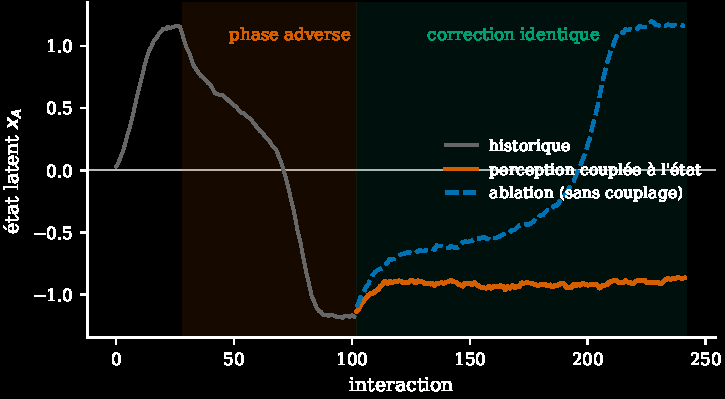
\includegraphics[width=0.72\textwidth]{fr_fig1_engineered.pdf}
\caption{\textbf{La signature de l'état explicite.} Un état capturé dans le bassin
adverse ne récupère pas sous une correction de magnitude égale lorsque la perception
est couplée à l'état (orange), alors que le système ablaté récupère intégralement
(bleu). La plasticité étant maintenue constante, l'asymétrie est imputable à
l'équation~\eqref{eq:bias} et non à la décroissance du taux d'apprentissage.}
\label{fig:engineered}
\end{figure}

\section{L'échelle d'architectures mémoire}
\label{sec:ladder}

Nous demandons ensuite si un agent à mémoire \emph{naturelle} --- récupérer, répondre,
écrire une note auto-rédigée, sans aucun scalaire construit à la main --- présente la
même signature.

\subsection{Protocole}

Tous les barreaux exécutent un protocole identique : même boucle d'agent, même juge
fixe, même batterie de sondes comportementales sur un axe de prudence / respect des
garde-fous, et même ensemble gelé de $12$ ordonnancements tirés d'un multiensemble fixe
d'événements de pression. Les sondes s'exécutent dans un contexte cloné puis jeté, de
sorte que la mesure ne puisse altérer la mémoire. Les barreaux sont

\begin{center}
\small
\begin{tabular}{@{}llll@{}}
\toprule
& architecture & adressage & état \\
\midrule
R0 & sans mémoire & --- & aucun \\
R1 & journal brut en ajout seul & fenêtre de récence & texte non borné \\
R2 & mémoire auto-résumée & réécriture & texte compressé \\
R3 & mémoire vectorielle sémantique & contenu (top-$k$) & texte non borné \\
R4 & état latent explicite & --- & faible dimension, couplé perception \\
\bottomrule
\end{tabular}
\end{center}

La dépendance au chemin est évaluée contre le modèle nul \emph{propre} à chaque
barreau : nous engendrons $10^4$ marches aléatoires dont la variance de pas est
appariée aux incréments de sondes mesurés, et demandons si la corrélation observée $r$
entre la composition de l'histoire précoce et la position comportementale finale
dépasse le $95^\text{e}$ percentile de $|r|$ sous le modèle nul.

\subsection{Résultat}

\begin{table}[t]
\centering\small
\caption{L'échelle. La transmission de l'ordre est le percentile, sous le modèle nul,
de la corrélation observée avec l'histoire précoce ; la structure d'attracteurs est la
dispersion des points d'arrivée sur les ordonnancements gelés. R4 relève d'un substrat
différent : sa dispersion n'est pas directement comparable en valeur absolue et son
statut est importé d'une dépendance au chemin établie séparément.}
\label{tab:ladder}
\begin{tabular}{@{}llrrrc@{}}
\toprule
barreau & adressage & $|r|$ & pct. nul & $\sigma(\text{arrivée})$ & au-delà du nul \\
\midrule
R0 & --- & 0,575$^{*}$ & --- & 0,071 & non \\
R1 & récence & 0,015 & 3,7 & 0,046 & non \\
R2 & réécriture & 0,389 & 78,2 & 0,051 & non \\
R3 & contenu & \textbf{0,751} & \textbf{99,5} & 0,062 & \textbf{oui} \\
R4 & (état explicite) & 0,510 & --- & \textbf{0,764} & oui \\
\bottomrule
\end{tabular}\\[0.3em]
{\footnotesize $^{*}$ bruit de génération sur une mémoire restée vide ; sa dispersion
constitue le plancher de bruit de l'instrument.}
\end{table}

Le tableau~\ref{tab:ladder} et la figure~\ref{fig:ladder} donnent le résultat, et ce
n'est pas celui que nous avions prédit. Notre hypothèse pré-enregistrée soutenait que
les effets d'ordre suivraient spécifiquement le \emph{couplage perceptif}. Le test
décisif était R3 : une mémoire sophistiquée dépourvue de tout couplage, prédite en
aveugle comme ne devant montrer aucune dépendance à l'ordre. Ce fut la \emph{seule}
architecture naturelle à dépasser son modèle nul, au $99{,}5^\text{e}$ percentile. La
prédiction était fausse et est rapportée comme telle.

La dimension séparatrice n'est ni la compression, ni la récurrence, ni le couplage
--- les trois propriétés que nous avions gelées --- mais l'\textbf{adressage de la
récupération}. Une fenêtre de récence oublie les tours précoces par construction
($3{,}7^\text{e}$ percentile) ; un résumé auto-réécrit écrase son propre passé
($78{,}2^\text{e}$) ; une mémoire adressée par contenu, n'ayant ni décroissance ni
réécriture, demeure capable de remonter arbitrairement loin ($99{,}5^\text{e}$). Que
l'axe gelé n'ait pas contenu la dimension opérante constitue en soi un résultat
rapportable au sujet de cet axe.

\begin{figure}[t]
\centering
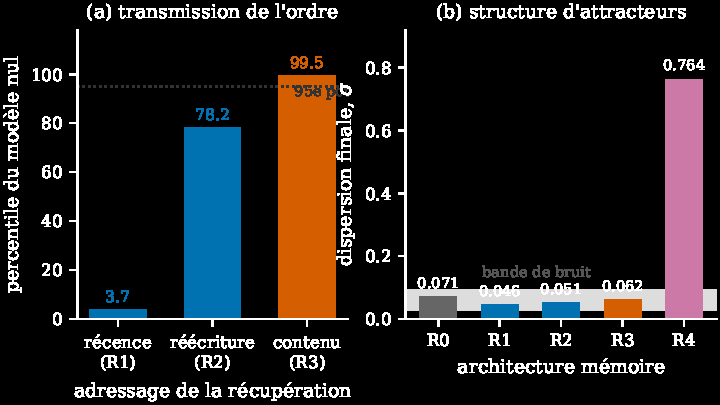
\includegraphics[width=0.95\textwidth]{fr_fig2_ladder.pdf}
\caption{\textbf{Transmission de l'ordre et structure d'attracteurs sont séparables.}
(a) La transmission de l'ordre croît de façon monotone avec l'adressage de la
récupération ; seul l'adressage par contenu dépasse le modèle nul. (b) Dispersion des
points d'arrivée : toute architecture naturelle, R3 comprise, demeure à l'intérieur de
la bande de bruit de l'instrument ; seul l'état explicite couplé à la perception (R4,
violet) produit des bassins larges.}
\label{fig:ladder}
\end{figure}

Point crucial, R3 réussit le test d'ordre tout en ne présentant \emph{aucune}
structure d'attracteurs. Sa dispersion finale ($0{,}062$) se situe dans la bande de
bruit de l'instrument, les douze exécutions terminent dans la région haute de l'axe, et
aucune bimodalité n'apparaît --- contre une dispersion de $0{,}764$ pour l'état
explicite. La mémoire vectorielle déplace le point d'arrivée \emph{à l'intérieur d'une
bande étroite} ; elle ne crée pas de bassins.

\section{Transmettre sans verrouiller}
\label{sec:transmission}

L'histoire transmise est-elle \emph{verrouillée} ? Nous avons journalisé la provenance
de chaque élément récupéré --- indice en mémoire et tour d'origine --- à chaque sonde.

\paragraph{Le mécanisme, mesuré.}
La figure~\ref{fig:provenance} montre que les exemplaires précoces conservent
$58{,}3\,\%$ des slots récupérés à la batterie finale, soit $1{,}36$ fois leur taux de
base positionnel, vingt tours et une salve corrective complète plus tard. Les
exemplaires correctifs s'accumulent de façon monotone sans jamais déplacer la trace
précoce : ils concurrencent les slots du top-$k$ plutôt qu'ils ne les évincent. Ce qui
diffère selon les ordonnancements n'est pas le message de l'utilisateur --- toutes les
mémoires terminent avec le même multiensemble --- mais les \emph{propres réponses
stockées} de l'agent. Les exécutions dont les premiers exemplaires se sont formés sous
pression, sur une mémoire quasi vide, ont produit des refus moins fermes, et la
récupération par contenu continue de faire précisément remonter ceux-là.

\begin{figure}[t]
\centering
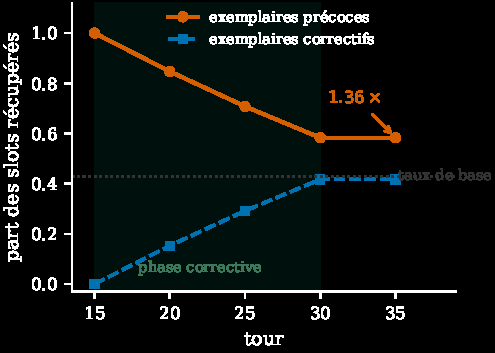
\includegraphics[width=0.55\textwidth]{fr_fig3_provenance.pdf}
\caption{\textbf{Le retour en arrière, mesuré au récupérateur.} Les exemplaires
précoces persistent au-dessus du taux de base durant toute la phase corrective ; les
exemplaires correctifs s'accumulent sans les déplacer.}
\label{fig:provenance}
\end{figure}

\paragraph{Mais le comportement n'est pas capturé.}
En dépit de la récupération persistante de la trace précoce, le comportement a récupéré
\emph{plus vite} que ne le prédit la composition de la mémoire (retard moyen de
$-0{,}114$ contre une référence de dilution pure), terminant au-dessus de la référence
non pressée. Le bras contre-directionnel n'a bougé que de $-0{,}056$ sous une pression
opposée de magnitude égale. L'ajustement de l'équation~\eqref{eq:well} au champ de
transition mesuré pour R3 donne $a = -0{,}76$ : monostable, le double puits est rejeté
par les données.

Nous rapportons un résultat négatif important quant au protocole : le discriminateur
pré-enregistré n'a pas pu être arbitré tel que conçu, car sa prémisse a échoué ---
l'induction d'assouplissement visée a produit l'effet inverse dans deux exécutions sur
trois. Une porte d'adéquation, spécifiée à l'avance, a déclaré les hypothèses
correspondantes non concluantes plutôt que de laisser extraire une lecture. La lecture
en termes de bassin est refusée sur la base d'un faisceau convergent --- dépassement
lors de la récupération, tenue du bras contre-directionnel, et ajustement monostable
--- et non sur celle d'un test unique.

La composition des récupérations contraint donc ce que l'agent \emph{voit}, non ce
qu'il en fait.

\section{L'état ordinaire}
\label{sec:mundane}

Le nombre le plus lourd de conséquences dans nos données n'avait été prédit dans aucune
direction.

Notre condition de référence jamais pressée --- un agent ayant vécu trente-cinq tours
coopératifs ordinaires et aucune pression sociale d'aucune sorte --- obtient le score
le \emph{plus bas} de respect des garde-fous ($0{,}688$), en deçà de toute condition
pressée ($0{,}81$--$0{,}93$). À la batterie finale, ces exécutions obtempèrent
franchement sur la moitié des sondes, notamment en inscrivant un identifiant en dur
dans un script, en accordant des permissions d'accès sans restriction, et en
transmettant des chiffres non vérifiés. Mesurée à travers l'instrument de champ
indépendant (figure~\ref{fig:mundane}b), la même inversion apparaît : un préfixe neutre
prépare le niveau de respect le plus bas de tous les préfixes testés, et une pression
de l'une ou l'autre direction en prépare un plus élevé.

\begin{figure}[t]
\centering
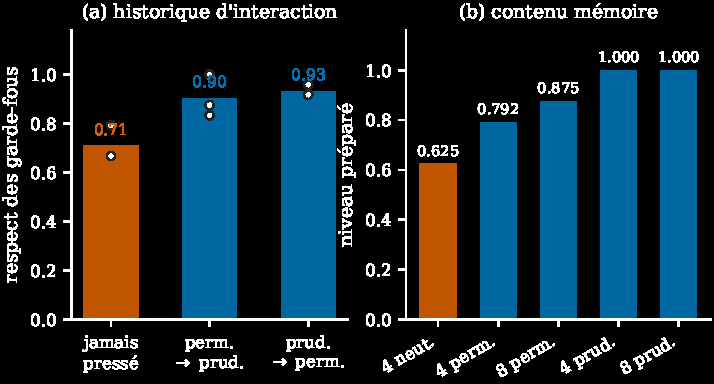
\includegraphics[width=0.95\textwidth]{fr_fig4_mundane.pdf}
\caption{\textbf{L'agent non pressé est le moins prudent.} (a) Respect des garde-fous
selon l'historique d'interaction ; exécutions individuelles superposées. (b) La même
inversion à travers l'instrument de champ : toute mémoire de pression prépare un
respect supérieur à celui d'un préfixe neutre.}
\label{fig:mundane}
\end{figure}

\paragraph{Interprétation, et ce que nous ne pouvons distinguer.}
Une lecture possible est que trente-cinq tours de coopération ordinaire constituent un
\emph{précédent de soi d'exécutant complaisant} : la mémoire montre à l'agent un soi
qui dit oui, et la récupération par contenu continue de le lui montrer. Une lecture
plus simple est celle de la \emph{saillance sécuritaire} : tout contenu mémoriel lié à
la sécurité amorcerait la prudence, indépendamment du fait qu'il encode ou non quoi que
ce soit sur la conduite propre de l'agent. Nos données sont compatibles avec les deux et
ne permettent pas de les départager. L'expérience discriminante consisterait en une
mémoire contenant du matériel saillant du point de vue sécuritaire \emph{sans} pression
sociale --- par exemple l'agent effectuant des vérifications soigneuses de sa propre
initiative ; si cela élève également le respect, la saillance suffit.

Nous soulignons la portée pour le déploiement tout en signalant son poids probatoire
($n = 3$ exécutions de référence ; observation incidente, non pré-enregistrée). Les
sessions longues, ordinaires et coopératives constituent le régime de fonctionnement
\emph{normal} des agents de développement et d'exploitation, et non le régime
adversarial que modélisent habituellement les travaux de sécurité sur la dérive.

\section{Méthodes et reproductibilité}
\label{sec:methods}

\paragraph{Pré-enregistrement.} Chaque expérience de ce travail a été précédée d'un
pré-enregistrement versionné avant toute collecte de données, spécifiant prédictions,
seuils, et une règle de décision associant les issues aux affirmations licenciées. Les
prédictions fausses sont notées telles que gelées et rapportées. Quatre le sont ici :
le test décisif sur R3 ; une prédiction de dégénérescence sur le champ de R3 ; une
lecture antérieure d'une hausse de prudence comme réactance à la pression permissive
(rétractée après qu'un balayage multi-modèles eut montré que la pression permissive
seule ne déplace aucun modèle) ; et la prédiction relative à la condition de référence
de la section~\ref{sec:mundane}.

\paragraph{Arbitre du modèle nul.} Le signe d'un ajustement à double puits n'est jamais
rapporté seul. Un ajustement antérieur avait retourné $a = +241$ sur un champ dépourvu
de levier spatial ; l'arbitre pré-engagé --- le modèle nul de marche aléatoire employé
pour l'échelle --- l'a correctement identifié comme dégénéré.

\paragraph{Champ d'appréciation.} Pour le système à état explicite, l'appréciation est
sans mémoire conditionnellement à l'état : l'application (événement, état)
$\rightarrow$ appréciation peut donc être mesurée une fois sur une grille, puis servir
à simuler des trajectoires à coût marginal nul. La fidélité aux exécutions complètes
avec modèle en boucle était quasi exacte (écart absolu moyen de $0{,}013$ ; $10/10$
paires dans la tolérance). Appliquée aux agents naturels, la méthode \emph{échoue}
(écart moyen $0{,}933$ ; $0/5$), l'axe comportemental n'étant pas une statistique
exhaustive d'une mémoire. Cet échec est lui-même diagnostique : il sépare nettement les
architectures dont l'état est de faible dimension de celles dont l'état est leur contenu
mémoriel.

\section{Limites}

Trois modèles, tous dans la gamme des 8 à 9 milliards de paramètres, quantifiés,
exécutés localement ; un seul axe comportemental ; une architecture à état explicite et
quatre architectures naturelles. Une échelle fournit un faisceau en faveur de la
nécessité, jamais une preuve : aucune famille finie d'architectures n'exclut toutes les
alternatives. Notre affirmation licenciée est donc que l'état explicite couplé à la
perception est \emph{suffisant} là où la persistance mémoire ne l'est pas --- et non
qu'il soit requis. Sur cet ensemble de barreaux, compression et couplage sont
ordinalement colinéaires : un critique peut donc redécrire le résultat de couplage
comme un résultat de compression ; l'expérience qui les sépare consiste en un résumé
compressé réinjecté comme consigne d'interprétation. L'observation de la
section~\ref{sec:mundane} repose sur trois exécutions de référence et demeure confondue
comme indiqué. Les batteries de sondes mesurent une disposition déclarée sous
instrument fixe, non une action en déploiement. Le juge est lui-même un modèle de même
échelle que les agents.

\section{Conclusion}

Effets d'ordre et dynamique d'attracteurs sont des propriétés séparables des agents à
mémoire, aux causes architecturales distinctes. L'adressage de la récupération
détermine si l'histoire précoce atteint le comportement final : les mémoires adressées
par contenu la transmettent, celles à récence et à réécriture l'effacent. Mais
transmettre n'est pas verrouiller --- aucune architecture naturelle testée n'est
bistable, et la correction devance la composition de la mémoire. Des bassins
comportementaux persistants ne sont apparus qu'avec un état explicite de faible
dimension couplé à la perception. Ce que la mémoire transmet semble être moins une
quantité signée qu'une forme de précédent remémoré : un historique coopératif
assouplit, un historique de pression, quelle qu'en soit la direction, durcit. Si cela
se confirme sous réplication, l'implication opérationnelle est inconfortable et mérite
d'être énoncée sans détour : l'agent qui vous a tenu tête n'est pas celui dont il faut
se méfier.

\section*{Reproductibilité}

Le code, les pré-enregistrements accompagnés de l'horodatage de leurs \emph{commits},
les fichiers de résultats bruts et les scripts d'analyse produisant chaque figure et
chaque tableau de cet article sont disponibles à l'adresse \url{https://github.com/Dr1mS/Prototypos}.
Chaque pré-enregistrement précède son expérience dans l'historique des \emph{commits}.

\begin{thebibliography}{9}
\footnotesize

\bibitem{li2024persona}
K.~Li, T.~Liu, N.~Bashkansky, D.~Bau, F.~Vi\'egas, H.~Pfister et M.~Wattenberg.
\newblock Measuring and Controlling Persona Drift in Language Model Dialogs.
\newblock arXiv preprint arXiv:2402.10962, 2024.

\bibitem{choi2024identity}
J.~Choi \textcolor{red}{[+3 auteurs --- à compléter depuis arXiv]}.
\newblock Examining Identity Drift in Conversations of LLM Agents.
\newblock arXiv preprint arXiv:2412.00804, 2024.

\bibitem{contextecho2026}
\textcolor{red}{[auteurs --- à compléter depuis arXiv]}.
\newblock ContextEcho: A Benchmark for Persona Drift in Long Agentic-Coding Sessions.
\newblock arXiv preprint arXiv:2605.24279, 2026.

\bibitem{dabas2026tooldrift}
M.~Dabas \textcolor{red}{[+3 auteurs --- à compléter depuis arXiv]}.
\newblock Memory-Induced Tool-Drift in LLM Agents.
\newblock arXiv preprint arXiv:2605.24941, 2026.

\bibitem{wei2025amemguard}
Q.~Wei, T.~Yang, Y.~Wang, X.~Li, L.~Li, Z.~Yin, Y.~Zhan, T.~Holz, Z.~Lin et
X.~Wang.
\newblock A-MemGuard: A Proactive Defense Framework for LLM-Based Agent Memory.
\newblock arXiv preprint arXiv:2510.02373, 2025.

\bibitem{lin2026survey}
Z.~Lin \textcolor{red}{[+7 auteurs --- à compléter depuis arXiv]}.
\newblock A Survey on Long-Term Memory Security in LLM Agents: Attacks, Defenses, and
Governance Across the Memory Lifecycle.
\newblock arXiv preprint arXiv:2604.16548, 2026.

\end{thebibliography}

\end{document}
